\documentclass[type=msc,colorback,accentcolor=tud8b,12pt,twoside,openright,bibliography=totoc,listof=totoc]{tudthesis}

% The following configuration file is greatly basen on a configuration file that was (as far as I know) developed by Waqas Abbas for his Master Thesis at TU-Darmstadt in 2017.

\usepackage{hyperref}
\usepackage{emptypage}
\usepackage[toc,page]{appendix}
% Handling chapters & section title alignment

% no indentation for new paragraphs
%\setlength{\parindent}{0pt}

% input encoding
\usepackage[utf8]{inputenc}

% font encoding
\usepackage[T1]{fontenc}

% german or english document
% \usepackage[ngerman]{babel}
\usepackage[english]{babel}

% set line spacing to 1.5
\usepackage{setspace}
\onehalfspacing

\usepackage{listings} %code highlighter
\lstset{
	literate={ö}{{\"o}}1
	{ä}{{\"a}}1
	{ü}{{\"u}}1
}
\usepackage{color} %use color
\definecolor{mygreen}{rgb}{0,0.6,0}
\definecolor{mygray}{rgb}{0.5,0.5,0.5}
\definecolor{mymauve}{rgb}{0.58,0,0.82}

\usepackage[T1]{fontenc}
\usepackage{selinput}
\SelectInputMappings{%
	adieresis={ä},
	eacute={é},
	Lcaron={Ľ},
}

%Customize the look
\lstset{ %
	backgroundcolor=\color{white}, % choose the background color; you must add \usepackage{color} or \usepackage{xcolor}
	basicstyle=\footnotesize, % the size of the fonts that are used for the code
	breakatwhitespace=false, % sets if automatic breaks should only happen at whitespace
	breaklines=true, % sets automatic line breaking
	captionpos=b, % sets the caption-position to bottom
	commentstyle=\color{mygreen}, % comment style
	deletekeywords={...}, % if you want to delete keywords from the given language
	escapeinside={\%*}{*)}, % if you want to add LaTeX within your code
	extendedchars=true, % lets you use non-ASCII characters; for 8-bits encodings only, does not work with UTF-8
	frame=single, % adds a frame around the code
	keepspaces=true, % keeps spaces in text, useful for keeping indentation of code (possibly needs columns=flexible)
	keywordstyle=\color{blue}, % keyword style
	% language=Octave, % the language of the code
	morekeywords={*,...}, % if you want to add more keywords to the set
	numbers=left, % where to put the line-numbers; possible values are (none, left, right)
	%numbersep=5pt, % how far the line-numbers are from the code
	numberstyle=\tiny\color{mygray}, % the style that is used for the line-numbers
	xleftmargin=2.5em,
	xrightmargin=1em,
	framexleftmargin=2em,
	rulecolor=\color{black}, % if not set, the frame-color may be changed on line-breaks within not-black text (e.g. comments (green here))
	showspaces=false, % show spaces everywhere adding particular underscores; it overrides 'showstringspaces'
	showstringspaces=false, % underline spaces within strings only
	showtabs=false, % show tabs within strings adding particular underscores
	stepnumber=1, % the step between two line-numbers. If it's 1, each line will be numbered
	stringstyle=\color{mymauve}, % string literal style
	tabsize=2, % sets default tabsize to 2 spaces
	title=\lstname % show the filename of files included with \lstinputlisting; also try caption instead of title
}

%javalanguage
\definecolor{darkgray}{rgb}{.4,.4,.4}
\definecolor{purple}{rgb}{0.65, 0.12, 0.82}

%define Javascript language
\lstdefinelanguage{JavaScript}{
	keywords={typeof, new, true, false, catch, function, return, null, catch, switch, var, if, in, while, do, else, case, break},
	keywordstyle=\color{blue}\bfseries,
	ndkeywords={class, export, boolean, throw, implements, import, this},
	ndkeywordstyle=\color{darkgray}\bfseries,
	identifierstyle=\color{black},
	sensitive=false,
	comment=[l]{//},
	morecomment=[s]{/*}{*/},
	commentstyle=\color{purple}\ttfamily,
	stringstyle=\color{red}\ttfamily,
	morestring=[b]',
	morestring=[b]"
}

\lstset{
	language=JavaScript,
	extendedchars=true,
	basicstyle=\footnotesize\ttfamily,
	showstringspaces=false,
	showspaces=false,
	numbers=left,
	numberstyle=\footnotesize,
	numbersep=9pt,
	tabsize=2,
	breaklines=true,
	showtabs=false,
	captionpos=b
}


% multiple rows inside a table
\usepackage{multirow}


% consistent text for graphics
\usepackage{psfrag}

% bibliography with biblatex and biber backend
\usepackage[style=alphabetic,backend=biber]{biblatex}

% same style for URLs
\urlstyle{same}

% title not italic
\DeclareFieldFormat{title}{#1\isdot}

% colon between author and title
\renewcommand{\labelnamepunct}{\addcolon\space}

% use semicolon when multiple authors
\renewcommand{\multinamedelim}{\addsemicolon\space}

% seperate last author with semicolon
\renewcommand{\finalnamedelim}{\addsemicolon\space}

% format name
%\DeclareNameFormat{default}{\usebibmacro{name:last-first}{#1}{#4}{#5}{#7}\usebibmacro{name:andothers}}

% text for url
\DefineBibliographyStrings{ngerman}{urlseen={abgerufen am}}

% biblatex

\addbibresource{bibliography.bib}

% properly underlined url in bibliography
\usepackage{url}

% adds align command
\usepackage{amsmath}

% use graphics
\usepackage{graphicx}
\graphicspath{{gfx/}}
%\setinstitutionlogo{Images/dsp_logo.jpg}

% display pics next to each other, don't use older subfigure package
\usepackage{subfig}

% use nicer tables with footnotes
\usepackage{ctable}
\setupctable{
captionskip=0pt, framerule=0pt, nostar,
center, framesep=0pt, pos=tbp,
continued=(continued), maxwidth=0pt, super,
doinside={}, mincapwidth=0pt, table,
framebg=1 1 1, nonotespar, botcap,
framefg=0 0 0, nosideways, width=0.9\textwidth
}

% force all floats to render with \FloatBarrier
\usepackage{placeins}

% acronyms and nomenclature
\usepackage[acronym, toc, nonumberlist]{glossaries}

% links within latex


% break long URLs in toc
\usepackage{breakurl}

\usepackage{array}
\newcolumntype{L}[1]{>{\raggedright\let\newline\\\arraybackslash\hspace{0pt}}m{#1}}
\newcolumntype{C}[1]{>{\centering\let\newline\\\arraybackslash\hspace{0pt}}m{#1}}
\newcolumntype{R}[1]{>{\raggedleft\let\newline\\\arraybackslash\hspace{0pt}}m{#1}}

\setcounter{secnumdepth}{3}
\setcounter{tocdepth}{2}

% set \emph to display text italic
\DeclareTextFontCommand{\emph}{\textit}

%checkmarks for table
%\usepackage{amssymb}% http://ctan.org/pkg/amssymb
\usepackage{pifont}% http://ctan.org/pkg/pifont
\newcommand{\myes}{\ding{51}}%
\newcommand{\mno}{\ding{55}}%
\renewcommand{\emph}{\textit}%


\begin{document}
	
	\pagenumbering{roman}
	% Title page

% #1: English title
% #2: German title
% fromat: \thesistitle{english title}{german title}
\thesistitle{A Debugging Tool for Javascript Reactive Libraries}{}
% Name of Author
\author{Waqas Abbas}

% Dept name
% logo of included for thesis thesis

\department{Fachbereich Informatik}

% Group name. {leave it empty}
\group{Reactive Programming Technology}

% In date
% \date{21.03.2011}
\date{05.06.2017}

% #1: Name of Professor
% format: referee{prof 1}{prof 2}{prof 3}
% leave other twoo options empty
\referee{Prof. Dr. Guido Salvaneschi}{M.Sc. Pascal Weisenburger}{}
		\makethesistitle
		
		\chapter*{Ehrenw\"ortliche Erkl\"arung}
	Hiermit versichere ich, die vorliegende Bachelorarbeit ohne Hilfe Dritter und nur mit den angegebenen Quellen
    und Hilfsmitteln angefertigt zu haben. Alle Stellen, die aus den Quellen entnommen wurden, sind als solche
    kenntlich gemacht worden. Diese Arbeit hat in dieser oder \"ahnlicher Form noch keiner Pr\"ufungsbeh\"orde vorgelegen.
    Die schriftliche Fassung stimmt mit der elektronischen Fassung \"uberein.
	\vspace{1.5cm}
	
	\noindent Darmstadt, den 02. Januar 2018\hfill Benedikt Gross
	%\chapter*{Declaration of Authorship}

I herewith formally declare that I have written the submitted thesis independently. I did not use any outside support except for the quoted literature and other sources mentions in the paper. I clearly marked and separately listed all of the literature and all of the other resources which i employed when producing this academic work, either literally or in content. This thesis has not been handed in or published before in the similar form. Written version of this thesis corresponds to the electronic version.

\vspace*{3cm}
\noindent
\begin{tabular}{c} Darmstadt, 05 June 2017\\\rule{5cm}{1pt} \\ (Place, Date)\end{tabular}  \hfill \begin{tabular}{c} \\ \\ \rule{5cm}{1pt} \\ (Waqas Abbas)\end{tabular}
	\cleardoublepage
	
	\begin{abstract}
			Abstract
	\end{abstract}
	
	\cleardoublepage
	\tableofcontents


	\pagenumbering{arabic}
	\chapter{Introduction} \label{ch:Introduction}
Introduction Header Placeholder

\section{Background}
% Reactive Inspector and previous CRI mentioned

\section{Motivation}
% increase usablity of CRI
% advance to eventually be used in production environment


\section{Our Contribution}

In the last two sections, we introduced reactive systems, ...


As a summary, this thesis makes the following contributions:

\begin{itemize}

	\item Item 1
	\item Item 2
	

\end{itemize}


\section{Outline}

Outline Placeholder

%	\cleardoublepage
	\chapter{State of the Art} \label{chap:State of the Art}
% introduction

\section{Implementation of Reactive Systems}
	\subsection{Reactive Programming}
	%"Reactive programming provides dedicated language abstractions for reactive software. Reactive programming relieves developers from manually updating outputs when the inputs of a computation change, it overcomes a number of well-know issues of the Observer design pattern, and it makes programs more comprehensible." [github, rxScala guido] Its also declarative instead of imperative.
	% reactive programming is in general not asynchroneous but it can be used in async context.? (waqas says something different for RXjs)
	% observables, difference to Observer design pattern:
		% observables in a reactive system return/provide multiple values (a stream) instead of just the current state.
		% "Observables provide abstractions over a stream of events. Promises are synchronous executables with a single return value, whereas observables are asynchronous executables that return multiple values over time." [pradeep]
		%"The data produced by the producer is stored in observable which the consumer consumes."[Pradeep]
	% observables are also called signals[wikipedia] = values that vary over continuous time -> or in RxJs Observables, Bacon Properties
	% events = events which have occurrences at discrete points in time -> RxJs Subject, Bacon EventStream
	% "observables" are functions that tie an observer to a producer. A producer creates values over time. An observer reacts to the values of a producer and notifies all subscribers (in a push based system).
	%operators: "Each operator outputs an another observable without modifying the original data streams." [Pradeep]
	% push and pull based: 
		%"Push-based systems take events and push them through a signal network to achieve a result. Pull-based systems wait until the result is demanded, and work backwards through the network to retrieve the value demanded." https://en.wikipedia.org/wiki/Functional_reactive_programming
	% cold and hot observables https://medium.com/@benlesh/hot-vs-cold-observables-f8094ed53339
			% -> author: "RxJS 5+ Lead, Software Engineer at Google, RxWorkshop.com. Own view, not the companies"
		% cold: the subscribe call creates the producer - one producer (e.g. a websocket raising events) is created for each call to subscribe, it gets destroied if the observer unsubscribes -> unicast
		% hot: all calls to subscribe (usally) share one producer - multicast
		% Rx Subjects - functions as both observer and observable, multicast but will terminate if the last subscriber is unsubscribed, can not be reused after termination or if in error state. "It multicasts. All observers passed to it via `subscribe()` are added to an internal observers list."
			% "Armed with our Rx Subject above, we can use a bit of functional programming to make any “cold” observable “hot”:
			%function makeHot(cold) {const subject = new Subject();cold.subscribe(subject); return new Observable((observer) => subject.subscribe(observer));}
			%Our new `makeHot` method will take any cold observable and make it hot by creating a subject that is shared by the resulting observable."
			% in RxJs that is e.g. publish or share
	
	\subsection{RxJs and BaconJs}
	% Though there are other Javascript implementations of the reactive design pattern like https://github.com/stoeffel/awesome-frp-js,
	% kefir, cyclejs
	% this thesis focuses on RxJs and BaconJs, because these are the one the extension currently supports.
	
	%RXjs
	%var button = document.querySelector('button');
	%Rx.Observable.fromEvent(button, 'click')
	%.throttleTime(1000)
	%.scan(count => count + 1, 0)
	%.subscribe(count => console.log(`Clicked ${count} times`));
	% The essential concepts in RxJS which solve async event management are:
	%Observable: represents the idea of an invokable collection of future values or events.
	%Observer: is a collection of callbacks that knows how to listen to values delivered by the Observable.
	%Subscription: represents the execution of an Observable, is primarily useful for cancelling the execution.
	%Operators: are pure functions that enable a functional programming style of dealing with collections with operations like map, filter, concat, flatMap, etc.
	%Subject: is the equivalent to an EventEmitter, and the only way of multicasting a value or event to multiple Observers.
	%Schedulers: are centralized dispatchers to control concurrency, allowing us to coordinate when computation happens on e.g. setTimeout or requestAnimationFrame or others.
	%"The subscribers are not locked in a synchronous request and there can be an infinite sequence of next emissions from the observables to the observer." [Pradeep] although subscribing is in general a synchroneous operation.
	%"completed and error functions	being defined at the observer, which are invoked by the observable on respective events. This lets the observer know that an observable has exhausted sending values, or an error has occurred	when performing an operation on the observable." [Pradeep]
	%"Subjects can be both observable and an observer[37]. It is a special type of observable which	allows values to be multicasted to many observers" [Pradeep]
	%"Unsubscribing is an optional feature in RxJS as RxJS handles this by default but it makes sense to unsubscribe manually by a user if the source observable is emitting the values continuously and the user does not need values after a specific point of time." [Pradeep]
	%"With the support of RxJS, we can convert multiple values, arrays, events into observables."[Pradeep]
	% - current version in development 6.0.0-alpha.2, stable: 5.5.6
	% - github stats 31.1.2018 18:22 for current active version (they changed repositories multiple times): watch: 387 star: 10,540 fork: 991 contributors: 185 but since they changed the repository the total numbers for all versions are much higher.
	% licence: Apache 2.0 latest commit: 30.01.2018
	% first release on github: version 2.2.0 01.03.2013
	
	%Baconjs: 
	%Generally, this is how you implement an app with Bacon.js. Capture input into EventStreams and Properties - Transform and compose signals into ones that describe your domain. - Assign side-effects to signals.
	%EventStreams (distinct events) and Properties (values that change over time). 
	%$("#username input").asEventStream("keyup").map(function(event) { return $(event.target).val() }).toProperty("")
	% "In Bacon, these are two flavors of Observables. EventStreams and Property are two basic concepts	of Bacon.js that are basically known as events and behaviours in the literature of FRP." [waqas]
	% - BaconJS does not have cold observables [ref baconjs github - For RxJs Users]
	% - "Error handling is also a bit different: the Error event does not terminate a stream. So, a stream may contain multiple errors. To me, this makes more sense than always terminating the stream on error; this way the application developer has more direct control over error handling. You can always use stream.endOnError() to get a stream that ends on error!" [baconjs github]
	% - it has the "spy" feature which greatly reduces the required effort to create complementary tooling like CRI or RxFiddle. It can also be used to easily create extensive logging.
	% - created because "Bacon.js exists largely because I got frustrated with RxJs, which is a good library, but at that time didn't have very good documentation and wasn't open-source. Things have improved a lot in the Rx world since that. Yet, there are still compelling reasons to use Bacon.js instead. Like, for instance, more consistent stream/property behavior and (arguably) simplicity of use." [baconjs github]
	% - current version 2.0.0
	% - github stats 31.1.2018 18:22: watch: 156 star: 5,839 fork: 328 contributors: 83
	% licence: MIT latest commit: 30.01.2018
	% -> has a smaller community than RxJs
	% first release on github: version 0.7.90 08.03.2017
	

	\subsection{Debugging Reactive Code}
	% due to reactive programming being declarative ... [github, guido rxScala]
	% short-comings of standard debuggers with reactive systems:
		% - stepping through reactive libarary code to track down bugs
		% - unconditional breakpoints in lambda functions will trigger to often to be useful 
		% - non-linear code execution makes step by step debugging hard -> "step over" is rarely useful and "step into" needs to be used multiple times for chained functions to iterate to the desired part, because "step over" will skip the whole line [verify with VS, IntelliJ, Webstorm, Chrome debugger].
		%- "lack of abstractions" and "mismatch in the mental model" [paper guido1]
		% - "Missing dependencies are hard to detect with traditional debuggers." [paper guido1 4.1]
	% - unit tests and do-debugging for Rx: https://msdn.microsoft.com/en-us/library/hh242967(v=vs.103).aspx to reduce the effort of adding do-statements each time a bug is tracked down, the developer can add logging functionality and use that in the do statement. https://shiny.rstudio.com/articles/debugging.html #"The Reactive log" where a visualization is later used on the log to create a simple dependency graph containing code pieces as nodes.
	% other systems that do
	% - Reactive Inspector for scala https://guidosalva.github.io/reactive-inspector/ is an extension of Scala IDE for Eclipse. Reactive Inspector is a project started and maintained by Guido Salvaneschi at the Software Technology Group - Technical University of Darmstadt, Germany and many people have contributed.
		% - Many features and the basic concepts that are implemented in CRI originate from RxScala Reactive Inspector. Dependency graph in the so called Reactive Tree, Tree History, History Queries, Reactive Breakpoints, Node search/dependencies/dependents. They are described in details in [Chapter: Previous CRI]
		% -"Tree Outline: Tree Outline In a large dependency graph it is sometimes hard to navigate the reactive tree. This view shows you at a glance where you are in the graph and helps you jump quickly to a different area of the graph."
	% - reference to rxfiddle in later section

\section{Previous and Related Work}
	\subsection{The Chrome Reactive Inspector}
		\subsubsection{Master Thesis by Waqas Abbas}
		% main focus of the thesis
			% - proof of concept
			% - how to intercept calls to reactive framework
			% - how to retrieve additional details for each node like the variable name via instrumentation of the source code to give context to observables shown in the dependency graph
		% implemented result of the thesis in short
			% - reactive breakpoints
			% - history queries
			% - Bacon support and partly support for Rx
			% - dependency graph, nodes, edges, zoom, highlighting of current node
			% - instrumentation, dynamically reloading of the page to intercept the javascripts for instrumentation
			% - first batch of test applications
			% -> focus on new implementation and prototypes of features and less on maintainability and reliability.
			% -> proof of concept
		
		\subsubsection{Master Thesis by Pradeep Baradur}
		% main focus of the thesis:
			% support for all RxJS operations and RxJS Subjects -> hard to implement, because there is no uniform way like the Bacon.spy method. For details on the general approach see [ref to pradeep thesis]. For source code see "rx-interception.js"
		% new features introduced:
			% - support for all operations and Subjects in RxJs
			% - loading of some CRI content scripts only when the CRI panel is opened. Istrumentation only when CRI panel is opened.
			% - find dependencys, dependents
			% - added many test applications
			% - improved reliability
			% - less focus on maintainability but move the project further to being usable in a production environment by adding framework feature support.
			% - rearranged UI, changed many styles to defaullt jquery-ui layout.
		
		\subsubsection{Merging previous efforts}
		%- took chrome-reactive-inspector 2 as base and merge all later developed features into it, piece by piece. manually copied changes by Pradeep from Waqas's repository. Hard to detect, changed to match other variable names before committing.
		% - uncompatible git histories - solvable but not much use since the files had separated so much in text character changes, though not so much in logic -> renames and splitting of files
		% - access to many global variables made tracking down dependencies of components hard with mixed contexts - some files with the window object corresponding to contentscripts in the same directory as files with a window object corresponding to the extensions window.
		%TODO: change tone to always present problems as general difficulties instead of shortcomings
		% - merged additional features of Abbas with framework support from Pradeep
		
		\subsubsection{"Special Curicumstances"}
		% demo version of jalangi
		% instrumenting files via scanning the html for script tags
		% -> will not work for module loaders like require.js or ecma6
		% -> will not work with bundled javascript code - but since in development there should be a non bundled version available not 
		% a big problem in javascript. But for Typescript since the extension does not support it and when compiling there may already be bundling in place. (#add some text from future here#)
		
		% Shared context through "new Function" that breaks the separation enforced by chrome. To increase consistency and prevent different execution contexts the previous eval was replaced with "new Function" but this does not reduce the security risk.There are other options to execute scripts from a chrome extension but since some of the extension scripts need to share the Rx or Bacon object with the inspected pages javascript files there is no other way. ofcorse that breaks the normal isloated world and intodruces a new set of problems like conflicting names. The security risk involved in executing a foreign script in a "trusted" extension context could be reduced if a sandbox was used as described in https://developer.chrome.com/extensions/sandboxingEval. Then all the inspected pages content scripts and some special recording scripts could be executed in that sandbox and transmitt the recorded nodes back via message passing.
		% - Dangers of using eval -> execution in current context. if called from other function, "this" might change. Function() for global with window passed to execute in original context.
		%- Note that  files that are not selected for instrumentation will still generate nodes in the graph, because the Rx and Bacon frameworks will still record interactions, just the information provided by instrumentation is missing.
		%- The Bacon and Rx scripts are prevented from loading so the extensions own files can be used. This is accomplished by filtering all referenced js files in the inspected page for any Bacon or Rx library files and excluding them from the loading process. They need to match version exactly though. This is necessary to guarantee that both work with the same Rx/Bacon object.
	

	\subsection{RxFiddle}
	% RxFiddle is the main competitor with CRI since it is the only other tool (that we are aware of) that tackels debugging for reactive javascript systems. Currently the only reactive framework that is supported is RxJs.
	% features of RxFiddle
	% limitations: 'one of the limitations of RxFiddle is ... which we tackeld in this work.
		% - requires more setup to use with web sites that have DOM logic and applications with more than one Javascript files, although it is possible according to the author [ref rxfiddle attached].
		% - the variable names in the source code are not displayed in the ui. RxFiddle instruments RxJs to collect its data, not the source code itself like CRI.
		% - fast updating observables like "interval" since each value update creates a new marble for the observable, the view becomes encoumbered fast with this type of observables. As of this moment CRI also generates one or more steps for each update (if the node is not explicitly excluded), but it is easier to examine the value of a node in the first or last few steps (jump to the step and use the next/previous button). CRI can also query the result which provide means to cope with large dependency graphs or histories. In RxFiddle the limitating factor for the fine grained stepping is the available space and resulting overplotting of the value-marbles since the examination is implemented via tooltips on mouseover. For performance comparison see [Evalutation chapter section Performance Improvements].
		% - like the author explained in "https://github.com/hermanbanken/RxFiddle/issues/6" the web app can not work with large applications properly. The displaying of large applications in one graph is hard for both tools [reference to Contributions chapters], but RxFiddle needs more spaces for a single reactive operator than CRI. A large dependency graph with descriptive nodes is easier to examine than a large marble diagram that only shows information on nodes in tooltips except in the details view of a currently selected node so finding the desired node/operation is not as easy. RxFiddle also has performacne issue while rendering huge diagrams according to the author. RxFiddle would porbably need another view to appropiately cope with such large applications to help the user navigate and give an overview, although for mid-sized applications the graph on the left side where a user can choose which operation to examine can serve this purpose - As mentioned earlier RxFiddle does not porvide variable names which may lead to confusion of nodes if similar observables are in the same application.
		% As of now, CRI does not support multiple variables having the same name. The author describes some other options like priority ranking in the issue [ref].
		% - as mentioned erlier RxFiddle onyl supports RxJs while CRI also supports Bacon.js
	% - The author plans to support multiple collectors in the future for web applications, RxScala, RxJava, RxSwift and/or RxNet (source: "https://rxfiddle.net/tutorials.html#attached") which would provide the necessary data collection on one of these platforms and transmit this data to the RxFiddle tool/web-application to be able to use the same debugging environment (RxFiddle) with any of these platforms.



% end of state of the art chapter
%----------------------------------------------------------------------------
%latex sample code:



\begin{figure}[!h]
	\centering
	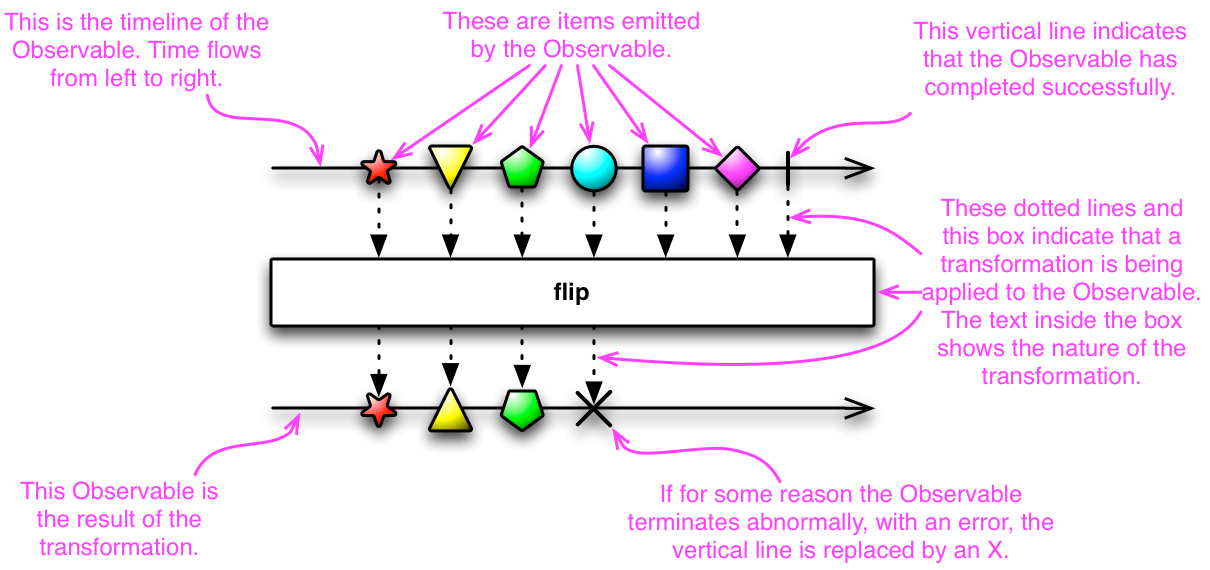
\includegraphics[scale=0.5,trim=0 0 0 0]{gfx/rxjs-reactive-pattern2.png}
	\caption{Reactive pattern \protect\cite{ReactiveXobservable}}
	\label{fig:rxjs-reactive-pattern}
\end{figure}

\textbf{Observable and Observer}\\
Placeholder

\textbf{Operators}
\label{subsec:Operators}\\

\textbf{RxJS Code Structure}\\
Placeholder
\begin{lstlisting}[language=JavaScript, caption=RxJS Simple Example, label={lst:RxJS_Simple_Example}]
// 1. Srouce Observable Creation
var sourceObservable = Rx.Observable.interval(1000);
// 2. Transformation by applying different operators
var transformedObservable = sourceObservable.map(function(x) {
		return x * 10;
	})
	.filter(function(x) {
		return x !== 20
	})
// OUTPUT
Next: 0
Next: 10
Next: 30
Next: 40
Next: 50
Completed
\end{lstlisting}

\subsection{Bacon.js}

\textbf{EventStream and Property}\\
Placeholder


	%\cleardoublepage
	\chapter{System Design} \label{chap:System Design}
In this chapter, we discuss high-level requirements for the system to be developed in this thesis and the system architecture is explained in detail. 
At the end of the chapter, we will discuss the design choices and system features.

\section{System Requirements}
The requirements for the system developed in this thesis are analyzed according to the idea that the dependency graph visualization and history improve the debugging process of an application based on reactive javascript libraries. We identified following requirements expressed in terms of functionalities available to the end user.

\leavevmode
\\
\textbf{Availability}
\\
The new system should seamlessly work and should be easily installable. Therefore, in order to reach many web developers, an extension for Google Chrome is being developed. 

\leavevmode
\\
\textbf{Visualisation of the Dependency Graph}
\\
While debugging, the developer should be able to see the dependency graph generated based on the developers' code. For the selected variable, all the dependents and dependencies of the variable should be shown in the graph, so that the developer understands the overview of the system. 
When the new values are generated, the graph should be automatically updated.

\leavevmode
\\
\textbf{Visualization of the History of the Dependency Graph}
\\
Once the graph is generated, the developer should be able to have a look at the graph at any arbitrary point in time. Thus, the whole history of the evolution of the graph can be visualized. It should also be possible for a developer to easily navigate through the time and observe the events such as node creation, node updates, dependency updates etc.

\leavevmode
\\
\textbf{Querying the History of the Graph}
\\
Depends on the size of the application, the size of graph grows. For large applications, it is not feasible to manually navigate through each step of the graph evolution. Therefore, a query language should be developed such that it makes easier for the developer to jump to specific points/events in the history. For example, the system should be able to jump to a specific point at which a node is created or updated.

\leavevmode
\\
\textbf{Breakpoints}
\\
Sometimes developer wants to halt the execution of the program by setting breakpoints at specific events. Our system should also provide developer an option to set breakpoints. For instance, it should be possible to set a breakpoint which is hit when a specific node is created or evaluated. 

\leavevmode
\\
\textbf{Helpers}
\\
System provides following additional features to the developer.

\begin{itemize}
	\item Search node by name in dependency graph.
	\item Pause or resume logging all values to the graph.
	\item Exclude selected nodes from logging values to the graph.
	\item An option to chose whether developer wants to print all the logged values to the console.
	\item Show dependents and dependencies of the selected node.
\end{itemize}

\section{System Architecture Overview}
The overall system design is illustrated in Figure~\ref{fig:system-design}. There are two system components: One is Chrome extension which provides extended debugging functionality for reactive applications and another one is client code which needs to be debugged. The general interaction between client code and extension is shown in the figure~\ref{fig:system-design}. 

\begin{figure}[!h]
	\centering
	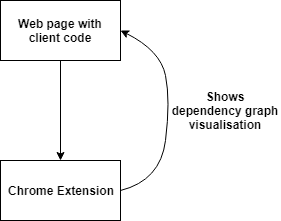
\includegraphics[scale=0.5,trim=0 0 0 0]{images/system-design.png}
	\caption{Overview of system design}
	\label{fig:system-design}
\end{figure}

The detailed system architecture is depicted in figure~\ref{fig:system-architecture}. The application is written using reactive javascript libraries(RxJS/BaconJS). Analyzer is a core component of the system. It helps the extension to catch all the events happening at both the libraries. In the current implementation, we support two reactive javascript libraries, RxJS and BaconJS. Analyzer analyzes all the events and passes the relevant information further to Chrome Reactive Inspector(CRI) panel. The information received by the panel is then stored in browser storage and also displayed as a dependency graph. CRI stores in-between steps or data to browser storage which helps developer for back in time debugging.

\begin{figure}[!h]
	\centering
	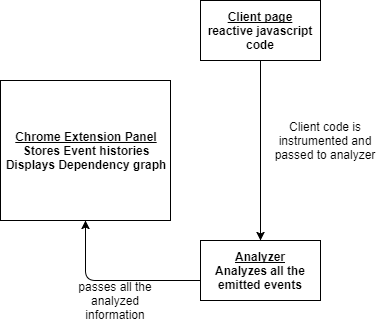
\includegraphics[scale=0.5,trim=0 0 0 0]{images/system-architecture.png}
	\caption{System Architecture}
	\label{fig:system-architecture}
\end{figure}

\subsection{Analyzer}
As we said earlier, Analyzer is the main building block of our system. It receives all the events and analyzes them. We will now look into how Analyzer is designed in detail.

RxJS library does not provide any interfaces to the developer for debugging purpose yet. But BaconJS provides a user an interface in the form of \textbf{Bacon.spy} method. Using this method, the developer can catch all the events emitted by clients' BaconJS code. Keeping these in mind, we designed Analyzer as shown in the figure~\ref{fig:analyzer-design}. 

\begin{figure}[!h]
	\centering
	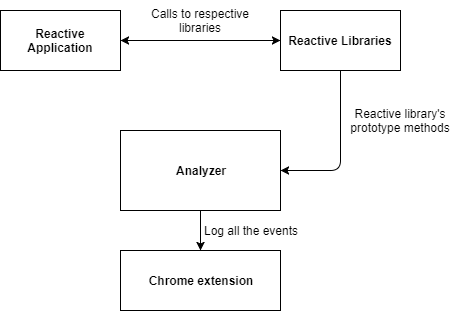
\includegraphics[scale=0.5,trim=0 0 0 0]{images/analyzer-design.png}
	\caption{Analyzer Design}
	\label{fig:analyzer-design}
\end{figure}

Here, we intercept and rewrite the required functions of both the libraries using prototype\cite{prototype}. Every object in javascript has an internal property called Prototype. Using this property, we are overriding required function calls of both libraries. We capture the required information and handover the call to original library call for further computations. Overriding all the function calls is not feasible and scalable. We observed that calls to various operators returned respective new observables. For instance, map operator returns MapObservable in RxJS. All types of observables call their respective subscribe functions which internally calls parent subscribe method. Thus, we only override parent subscribe method instead of individual subscribe methods. 

\section{System Architecture Details}
\subsection{Dependency Graph Visualization}
As explained earlier, dependency graphs help user visualize reactive applications. Each time-changing value is a node in the graph and a directed connection between two nodes if one node depends on another node. Consider the following RxJS code snippet for example. 
\begin{lstlisting}[language=JavaScript, caption=RxJS code example, label={lst:rxjs-code-example}]
var shortName = name.map(name => name.toLowerCase())
.filter(name => name.length < 5);

var bmi = weight.combineLatest(height, (weight, height) =>
Math.round(weight / (height * height * 0.0001))
);

var fullInfo = shortName.combineLatest(bmi);
\end{lstlisting}

In the above example, in Line 1, variable \textit{shortName} depends on variable \textit{name}. Similarly at Line 4, \textit{bmi} depends on both \textit{height} and \textit{weight}, at Line 8 \textit{fullInfo} depends on both \textit{shortName} and \textit{bmi}. The figure~\ref{fig:rxjs-dependency-graph-example}, how dependency graph looks after modeling it. This gives a very good overview of the reactive system and especially of the dependency therein. This should be of great help for developers to understand and analyze the reactive applications. 

\begin{figure}[!h]
	\centering
	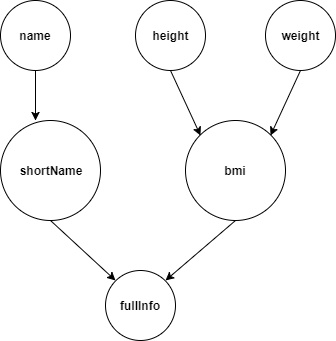
\includegraphics[scale=0.5,trim=0 0 0 0]{images/rxjs-dependency-graph-example.png}
	\caption{RxJS Dependency Graph Example}
	\label{fig:rxjs-dependency-graph-example}
\end{figure}

\subsection{Navigating through the Dependency Graph History}
The visualization of a graph is not only updated whenever an event occurs, but it also stores each stage when it changes. This gives the developer a possibility to navigate through the whole history. The developer can navigate through the history in following ways:
\\
\textbf{History Navigation}
\\
One way is to simply use back and forth buttons provided, which jump to the point in time directly before or after the current point of time.
\\
\textbf{Direct Access}
\\
History navigation may not be practical for application with large histories. The developer should be able to drag the slider and thus quickly jump to the desired point in time.
\\
\textbf{History Queries}
\\
A third and last option is to navigate through the history using provided query language. By entering valid queries, the developer can directly jump to the respective points in time when these events happened.

\subsection{Breakpoints}
In traditional debuggers, breakpoints are based on specific line or conditions. A breakpoint hits and halts the execution of program each time the code reaches specific line or encounters specific condition evaluates to true. These breakpoint type does not really fit well into the RP approach. Hence, RP specific breakpoints should be developed. They reuse the developed query language. The developer can enter a query, start to debug the application and the debugger will halt the execution each time the query matches. For instance, if developer enters a query \textit{NodeCreated[NodeId, 1]}, the debugger will halt the execution when a node with Id 1 is created. 

\subsection{Chrome extension}
In this thesis, we are implementing a debugger in the form of an extension to Google Chrome DevTools. With the help of chrome APIs, we can add more debugging capability to our extension. The extension adds a new panel to DevTools which provides all the features mentioned so far and also adds an options page where a user can use optional features. The same extension can be further extended and adapted to support other browsers like Mozilla Firefox\cite{firefox}.

\subsection{Scoping and other features}
The Jalangi framework, which we discussed earlier, instruments the given javascript code. It is performance hindering if we are instrumenting all other code which is not RxJS. So we provide scoping feature where a user can mention the file name to be instrumented. 
Another feature is, a user can search any existing node by name. This feature is useful when the dependency graph is large. The user can also figure out dependents and dependencies of any given node. As optional features, a user can exclude nodes to log events to the graph, can choose whether to log all the values to console. 

\subsection{Chrome Storage}
The Google chrome provides data storage facility to manage data for specific requirements\cite{chrome-storage}. There are options of local storage, session storage and an HTML5 storage available in chrome. The data is stored in the form of key-value pair. Local storage is persistent and has no expiration until the user deletes it explicitly. On the other hand, session storage is persistent only for current browser session and is erased when a browser is closed. We use local storage in our extension to store the data such as file name used for scoping feature, list of breakpoints, list of nodes to be excluded from logging events to the graph.


%	\cleardoublepage
	\chapter{Implementation} \label{chap:Implementation}
This chapter presents the implementation details of the CRI extension. In the first section, we present two alternative implementations of the CRI extension. The second section describes the significant data structures used by the extension. The communication in between different components of the extension is explained in the third section. The fourth section presents the developed query language and its usage. The last section describes the graphical user interface provided by the extension.

\section{CRI - Implementation Alternatives }
In this section, we present two possible implementations of CRI extension. To determine the best possible alternative is yet to discover by looking into the pros and cons of both alternatives and is mentioned as one of the possible future work. We tried our hands at both alternatives, but for the final version, we focused on the first alternative. So except this section, everything presented in this thesis is based on the first alternative. 


\subsection{Alternative - 1}


As described in section~\ref{subsec:Extending_Chrome_DevTools}, in Chrome DevTools extesnsion, page script and content script runs in two different execution contexts, and both have access to same DOM.
Figure~\ref{fig:system_implementation_detail_1} depicts component level details of the first alternative, where the user has an application with reactive
code to debug or analyse. Before execution takes place, the application code is intercepted by DevTools extension and the manipulated code is run in the browser which provides the same output as the original code.
All components residing within the big dotted round cornered box are run as a content script. \textbf{Interceptor} module is responsible for preventing JavaScript code in the target application from executing in the browser. For this purpose, we created a script that runs as a content script at document start. It uses \textbf{window.stop} to halt the normal loading of the web page to the browser. 
Then, we make a XHR(XMLHttpRequest) request to get the content of the target document. Replace the \textbf{type} attribute of all script tags with some custom string and write it to the document, this will stop the browser to execute that script. After that sequentially loads the JavaScript files and instruments them if required and injects them into the web page as a content script.
After instrumentation, when manipulated code runs in the browser then it invokes the Jalangi API on
different events like whenever any value is written to JavaScript variable.
Instrumentor receives JavaScript code from the interceptor module and performs instrumentation on a given JavaScript code with Jalangi library. Instrumentor returns instrumented code to the interceptor module. 


\begin{figure}[!h]
	\centering
	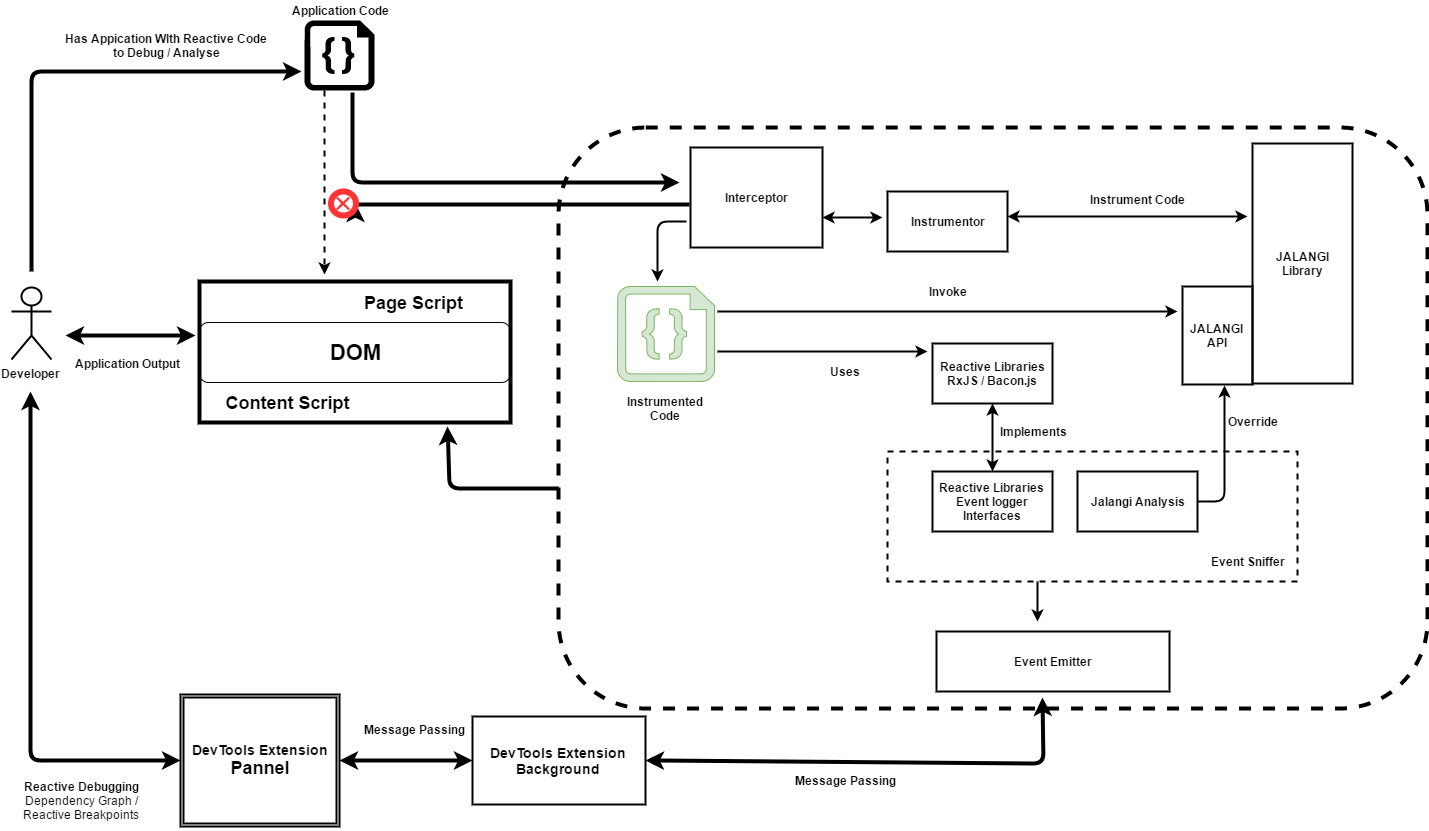
\includegraphics[width=\textwidth,height=\textheight,keepaspectratio]{gfx/SystemFlowDiagramDesign1.png}
	\caption{System Components Detail - Alternative 1}
	\label{fig:system_implementation_detail_1}
\end{figure}


\textbf{Event sniffer} comprises of two sub-components,
the first one contains the reactive library specific implementation to log all internal activities such as the creation of observable, and values emitted to subscribers.
The second sub-component of Event sniffer is Jalangi Analysis that overrides some methods of Jalangi API, which make it possible to map the reactive streams to the JavaScript variable name.
Event Emitter is also part of the content script, it receives events information from event sniffer, it changes them to defined message structure and passes this as a message to extension\textquotesingle s background page.
The communication in between content script, background page and extension panel is done with message passing  \footnote{\url{https://developer.chrome.com/extensions/messaging} , last accessed 24-05-2017}. 
Extension\textquotesingle s background page receives messages of a defined pattern from the event emitter and passes them to extension panel.
Similarly, background page also receives messages from extension panel and forwards them to content script.
Extension\textquotesingle s panel receives events information as a message from background page, parse those messages and responds according to the type of the message.
The message can be of type \textbf{saveNode} or \textbf{saveEdge}. If the message type is \textbf{saveNode} then we check whether it is an update to an existing node or it is a new node.
On receiving a message from the background page, extension panel update the dependency graph and save the graph state in the browser storage. Whenever the new state of dependency graph is saved to the browser storage, the step slider is also updated.
Finally, the developer sees the updated dependency graph, to which he can interact with by setting reactive break points or navigating through the history of the dependency graph. 







\subsection{Alternative - 2}  \label{subsec:Alternative_2}





\begin{figure}[!h]
	\centering
	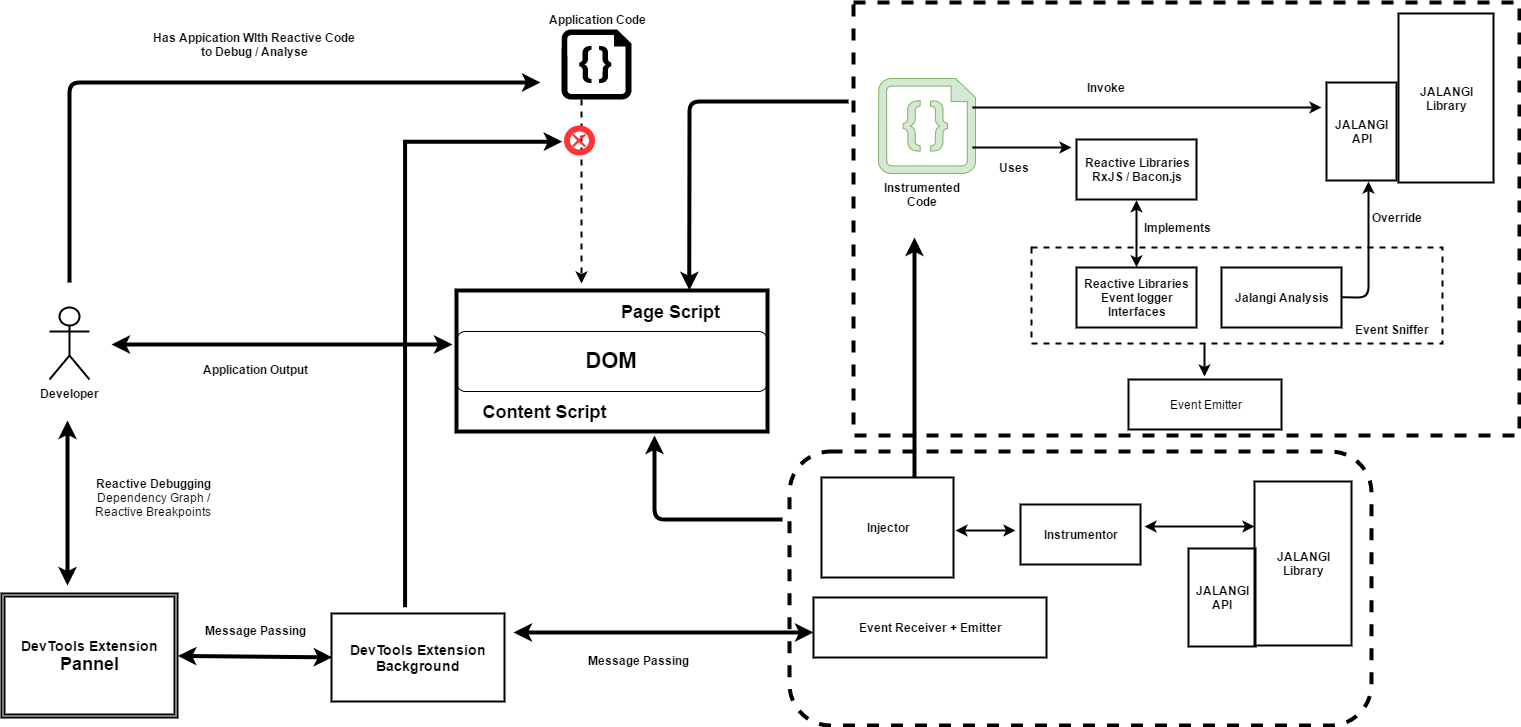
\includegraphics[width=\textwidth,height=\textheight,keepaspectratio]{gfx/SystemFlowDiagramDesign2.png}
	\caption{System Components Detail - Alternative 2}
	\label{fig:system_implementation_detail_2}
\end{figure}

Figure~\ref{fig:system_implementation_detail_2} presents the implementation details of the second approach. Most of the modules are common to the first option.
With this approach, instead of preventing the whole page from loading to the browser, we use \textbf{chrome.webRequest}\footnote{\url{https://developer.chrome.com/extensions/webRequest} , last accessed 25-05-2017} API in background page of the extension to only intercept the HTTP request to specific files that are defined in the field of the scoping feature.
Injector script is run as a content script by extension at the end of the document loading; it is responsible for getting target JavaScript files with XHR request and instrumenting it with Jalangi. 
All modules within the dotted square box are injected by injector script into the target web page as page scripts. Event sniffer works similarly as in the first approach.
Event emitter from the page script passes messages to \textbf{Event receiver + emitter} using \textbf{Window.postMessage()}\footnote{\url{https://developer.mozilla.org/en-US/docs/Web/API/Window/postMessage} , last accessed 25-05-2017}, which is then received in the content script by \textbf{Event receiver + emitter} .
From here onwards everything works as described in the first approach.
The noticeable differences in this method are as follows: 
1) instrumented code, and event sniffer modules run in page script context.
2) Intercepting of target JavaScript code is being done from background script of extension.




\section{Significant Data Structures}

There are two important data structures defined in CRI. The first one is used while sending a message from content script to the panel and the other is used while saving the history of dependency graph into Chrome storage. Listing~\ref{lst:imp_sig_data_structs} shows those significant data structures.

In CRI, the communication between content script (event emitter) and the panel has a defined data structure. 
The message object has two attributes named as \textbf{content} and \textbf{action}.
The \textbf{action} attributes define which type of event has occurred, and the \textbf{content} attribute contains detailed information about that message. Two important values of action attribute are \textbf{saveNode} and \textbf{saveEdge}.\\
In the case of \textbf{saveNode}, the \textbf{content} attribute contains \textbf{node} object and \textbf{node} object contains the following properties:\\
\begin{itemize}
\item \textbf{nodeId}: defines the unique id of the node.
\item \textbf{nodeType}: specifies the type of reactive variable, it can be observable, eventStream or property. Different reactive libraries have their own implementations for time-changing variables.
\item \textbf{nodeMethod}: determines the method name which results in this stream.
\item \textbf{nodeRef}: contains the JavaScript variable name, identified by jalangi. It can be empty in the case of intermediate streams; those are not directly assigned to a variable.
\item \textbf{nodeValue}: contains the current value of this reactive variable as a string.
\item \textbf{sourceCodeLine}: holds the line number from the source code, where this reactive variable is defined.
\end{itemize}
In the case when \textbf{action} attribute of the message is set to \textbf{saveEdge}, the \textbf{content} attribute contains edge object and \textbf{edge} object is defined by the following properties:\\
\begin{itemize}
\item \textbf{edgeStart}: The node id of the parent reactive variable, on which another reactive variable depends.
\item \textbf{edgeEnd}: The node id of the child reactive variable, which results in the application of some operator on parent reactive variable.
\item \textbf{edgeLabel}: The name of the operator which causes this dependency.
\end{itemize}

\begin{lstlisting}[language=JavaScript, caption=Significant Data Structures used by CRI, label={lst:imp_sig_data_structs}]
// Message object in case of dependency creation
{
	content: {
		"edgeStart": '',
		"edgeEnd": '',
		"edgeLabel": ''
	},
	action: "saveEdge",
	destination: "panel"
}

// Message object in case of new reactive stream defined / existing stream gets a new value
{
	content: {
		'nodeId': '',
		'nodeType': '',
		'nodeMethod': '',
		'nodeRef': '',
		'nodeValue': '',
		'sourceCodeLine': ''
	},
	action: "saveNode",
	destination: "panel"
}

// Data Structure for history of dependency graph
{
	"stageId": '',
	"stageEvent": '',
	"stageCurrentNode": '',
	"stageCurrentEdgeStart": '',
	"stageCurrentEdgeEnd": '',
	"stageData": {
		"nodes": [],
		"edges": []
	}
}
\end{lstlisting}

History of dependency graph is saved to chrome storage as an array of \textbf{stage} objects, and \textbf{stage} object comprises of the following properties. Each stage represents a single step of the history of the dependency graph.\\
\begin{itemize}
\item \textbf{stageId}: represents the id of the stage/step for the history of the dependency graph.
\item \textbf{stageEvent}: represents the event that causes this stage. (saveEdge, newNode, updateNode)
\item \textbf{stageCurrentNode}: represents the id of the current node. It is used to highlight a node in the dependency graph.
\item \textbf{stageCurrentEdgeStart}: If current stageEvent is saveEdge then this property contains the parent node id.
\item \textbf{stageCurrentEdgeEnd}: If current stageEvent is saveEdge then this property contains the child node id.
\item \textbf{stageData}: is an object that contains an array of all nodes and edges objects.
\end{itemize}

\section{Communication between Extension Components}

Since the content scripts run in the context of a web page and not the extension, they often need some way of communicating with the rest of the extension. In our case of CRI implementation, event sniffer script run as a content script. It has to forward the information about logged events from reactive libraries to the panel, which further reacts to those messages by updating dependency graph in the panel GUI and saving this information to browser storage for later access. Communication between extension components works by using message passing.
Two possible ways to communicate between extension components are simple one-time requests and long-lived connections\footnote{\url{https://developer.chrome.com/extensions/messaging} , last accessed 26-05-2017}.
We use long-lived connections because event sniffer would send messages continuously. Extension\textquotesingle s panel creates a channel to background script with the name \textbf{reactive-debugger} and adds listeners to receive messages from the background script.
Listing~\ref{lst:imp_comm_panel_code} shows the relevant code that panel script uses to create a connection with background script.


\begin{lstlisting}[language=JavaScript, caption=Panel Script to Communicate with Background, label={lst:imp_comm_panel_code}]
//Create a port with background page for continuous communication
var port = chrome.extension.connect({
	name: "reactive-debugger" //Given a Name
});
// Listen to messages from the background page
port.onMessage.addListener(function (message) {
	// Here we get message from background,
	// that gives us information about events like,
	// New reative variable is defined / Dependency established / New value of reactive stream
	
});
\end{lstlisting}

Listing~\ref{lst:imp_comm_background_code} shows the relevant code for background script to communicate with content scripts and panel script.
To handle incoming connections in background script, we set up an \textbf{extension.onConnect} event listener. When \textbf{extension.connect} is called from the panel script, \textbf{extension.onConnect} event is fired along with \textbf{runtime.port} object that we can use to send and receive messages through that connection. 
The \textbf{Event Emitter} module of CRI which also runs as content script send messages to background script by using \textbf{chrome.extension.sendMessage}, which is received by background script and forwarded to panel script.

As in the second alternative~\ref{subsec:Alternative_2}, the event emitter is injected into the web page context instead of running as content script so in this case the event emitter passes messages that it receives from event sniffer to the content script by using \textbf{window.postMessage} , which is received in content script \textbf{Event Reciever + Emitter} module.
Beside direct communication between extension components by message passing, there is an indirect communication which is being done by \textbf{chrome.storage} API already explained in section~\ref{subsec:Data_Storage_and_mgmt}.

\begin{lstlisting}[language=JavaScript, caption=Background Script to Communicate with Panel and Content Scripts, label={lst:imp_comm_background_code}]
chrome.extension.onConnect.addListener(function(port) {

	// Listens to all incoming messages
	// Message can be from content script or from panel
	chrome.extension.onMessage.addListener(extensionListener);
	
	// function to identify message source and forward its destination
	var extensionListener = function(message, sender, sendResponse) {
		// identify destination of message and forward it
		if (message.destination == "panel") {
			// message from content script so send it to panel
			port.postMessage(message);
		} else {
			if (message.tabId && message.content) {
				// message from panel and send to content script
				chrome.tabs.sendMessage(message.tabId, message, sendResponse);
			} else {
				// message from content script and send to panel script
				port.postMessage(message);
			}
		}
		sendResponse(message);
	}

	// Remove message listner when we close DevTools window
	port.onDisconnect.addListener(function(port) {
		chrome.extension.onMessage.removeListener(extensionListener);
	});
});
\end{lstlisting}


%\section{Dependency Graph Visualisation}
\section{The Query Language}  \label{sec:The Query Language}
Two important features of the CRI extension are based on query language.\\ 
A) Querying the dependency graph history after the execution of the application.\\ 
B) Setting reactive-programming specific breakpoints.\\ 

Let\textquotesingle s take a deeper look into the implementation of these two features.

The single commands are listed and explained in Table~\ref{table:imp_query_lang_for_history}.
The commands for feature \textbf{A} is based on nodeName\textquotesingle s and for feature \textbf{B} commands are based on nodeId\textquotesingle s.
In the first feature, extension gets the query when the user submits the query and it parses the submitted query with regular expressions. By applying regular expression we identify the query and its parameters. After identifying the query and its parameters, we apply the search operation to the data of dependency graph.
For the second feature, panel script stores the submitted queries in chrome storage and accesses it from the content script. The content script parses then those queries to apply breakpoint on the relevant place of the code.


\begin{table}[h!]
	\small
	\begin{center}
		\begin{tabular}{|l|l|p{3cm}|}
			\hline
			Command & Parameters & Description \\ \hline
				nodeCreated[nodeName] & nodeName: name of the node &  specific node is created \\ \hline
				nodeUpdated[nodeName] & nodeName:  name of the node &  specific node is updated, e:g node gets a new value \\ \hline
				evaluationYielded[nodeName][value] & \vtop{\hbox{\strut nodeName:  name of the node}\hbox{\strut value: a String}}   &  evaluation of specific node yields specific value \\ \hline
				dependencyCreated[nodeName1][nodeName2] &  \vtop{\hbox{\strut nodeName1:   name of the parent node}\hbox{\strut nodeName2:  name of the child node}} &  dependency between two specific nodes is created \\ \hline
			%	evaluationException[nodeName]  & nodeName: a name of a node &  evaluation of specific node throws an exception \\ \hline
		\end{tabular}
	\end{center}
	\caption{Commands of the Query Language}
	\label{table:imp_query_lang_for_history}
\end{table}




\section{Graphical User Interface}
\label{Graphical_User_Interface}
The graphical user interface of the debugger is Chrome DevTools panel view which can be opened just like any other panel in DevTools. The GUI is basically divided into six parts as shown in figure~\ref{fig:system_implementation_detail}. It can be activated by opening Chrome DevTools and navigating to \textbf{Reactive-Inspector} panel. 

The first part of the view just shows a text field to input the file names for scoping feature. In this field, one can enter JavaScript files name which should be considered for debugging. Multiple files name can be entered by separating them with a comma. If this particular field is left empty then the debugger will consider all JS files for debugging. The second part of the view contains some helper elements for the developer. One can search for a node by name within the dependency graph, the resultant node will be highlighted and remaining dependency graph will be faded out. One can also reset the current dependency graph and can start or pause debugging anytime. The current visualisation can also be downloaded as an image by pressing the \textbf{Download} button.


\begin{figure}[!h]
	\centering
	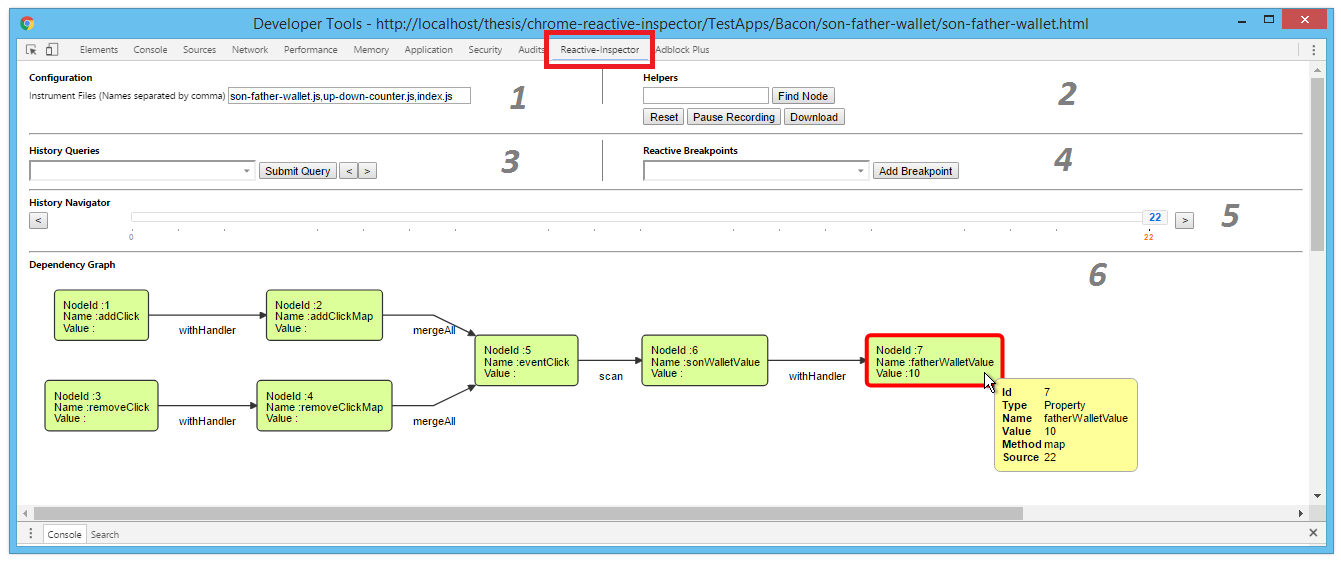
\includegraphics[scale=0.5,trim=0 0 0 0]{gfx/CRI-GUI.png}
	\caption{CRI - Graphical User Interface}
	\label{fig:system_implementation_detail}
\end{figure}

The third part of the view is to query the dependency graph, where
the developer can enter the queries explained in section~\ref{sec:The Query Language}. If a valid query is entered and the \textbf{Submit Query} button is pressed, the visualisation will jump to the first point in time at which the entered query matches. In the case of more results to a query, one can use navigation buttons available in this part to traverse through query results. The fourth part of the view is to set reactive breakpoints using the same query language that is used to search through the history of the dependency graph. 

The fifth part of the view is to navigate through the history of dependency graph with the help of a slider. One can navigate step-by-step with the help of buttons available on the left and right side of the slider. One can also use the mouse by dragging and dropping the pointer of the slider to any step. Every change to slider will result in changes to the dependency graph to a specific state. 

Last but not the least, the sixth part of the view contains the dependency graph. One can use the mouse to zoom in or out the current visualisation. Additional information to the nodes will be presented as a tooltip, if the developer hovers with the mouse over a specific node.The current node is highlighted with a red border around node box in the dependency graph.

The visualisation of the dependency graph is based on dagre-d3\footnote{\url{https://github.com/cpettitt/dagre-d3} , last accessed 25-05-2017}, which is a JavaScript library that acts as a front-end to dagre\footnote{\url{https://github.com/cpettitt/dagre} , last accessed 25-05-2017}, providing actual rendering using D3\footnote{\url{https://d3js.org/}, last accessed 25-05-2017}.
%	\cleardoublepage
	\chapter{Evaluation} \label{chap:Evaluation}
In this chapter, various case studies are introduced which demonstrate the use of an extension. They have been chosen in order to illustrate the important features of CRI, therefore the contributions of this thesis. We have collected examples written using RxJS and BaconJS libraries from the internet. We have evaluated the extension against several RxJS and BaconJS applications and we present the results in this section. We focus on features provided by our extension and evaluate those features with the applications. In the last section, we summarize and conclude the evaluation.

\section{Operators}
Operators play an important role in both libraries. Developers can use operators to transform, filter and for many other operations. To demonstrate how CRI helps developers to understand reactive applications, we have taken RxJS operators example code. This section also illustrates the evolution of dependency graph for the given example.

\subsection{RxJS - Operators}
In our example, we have selected \textit{map}, \textit{filter} and \textit{last} operators from RxJS library. One can find use case of other operators in RxJS official documentation\footnote{\url{http://reactivex.io/documentation/operators.html}}. Dependency graph generated by CRI after executing the program is shown in figure \ref{fig:rxjs-operators-dg}. In the following example~\ref{lst:rxjs-operators}, \textit{source} is an observable with values {1,2,3,4,5}. In line 3, \textit{map} operator is applied, which maps each values from an observable and adds 10 to each value and new \textbf{MapObservable} is created. At line 5, \textit{filter} operator filters the even values out of \textbf{MapObservable}. The \textit{last} operator at line 7 receives values 12 and 14 after applying filter operator and emits value 14 which the last value in observable. At line 9, subscriber \textit{subscribe} is subscribing to \textit{example} observable. Thus, \textit{subscribe} will receive value 14 and is printed to console in line 10.

\begin{lstlisting}[language=JavaScript, caption=RxJS - Operators example, label={lst:rxjs-operators}]
var source = Rx.Observable.from([1, 2, 3, 4, 5]);
// apply map, filter and last operator
var example = source.map(function (val) {
	return val + 10;
}).filter(function (num) {
	return num % 2 === 0;
}).last();
//output: "Last to pass test: 14"
var subscribe = example.subscribe(function (val) {
	return console.log("Last value: " + val);
});
\end{lstlisting}

\begin{figure}[!h]
	\centering
	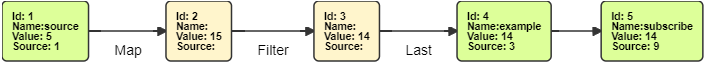
\includegraphics[scale=0.7,trim=0 0 0 0]{images/RxJS-operators/final.png}
	\caption{Dependency graph - RxJS Operators example}
	\label{fig:rxjs-operators-dg}
\end{figure}

As we said earlier, CRI helps the developer to understand the flow of reactive applications. For listing~\ref{lst:rxjs-operators}, evolution of dependency graph can be depicted as shown in figure \ref{fig:rxjs-operators-dg-evolution}. Developer can use the provided slider to navigate to and forth to visualize evolution of graph. In the first 3 steps, node \textit{source} is created and how the program runs internally after applying map and filter operator is depicted. In the last step, subscriber \textit{subscribe} is created which is subscribed to node \textit{example}. Thus, connection between \textit{example} and \textit{subscribe} exists.

\begin{figure}[!h]
	\centering
	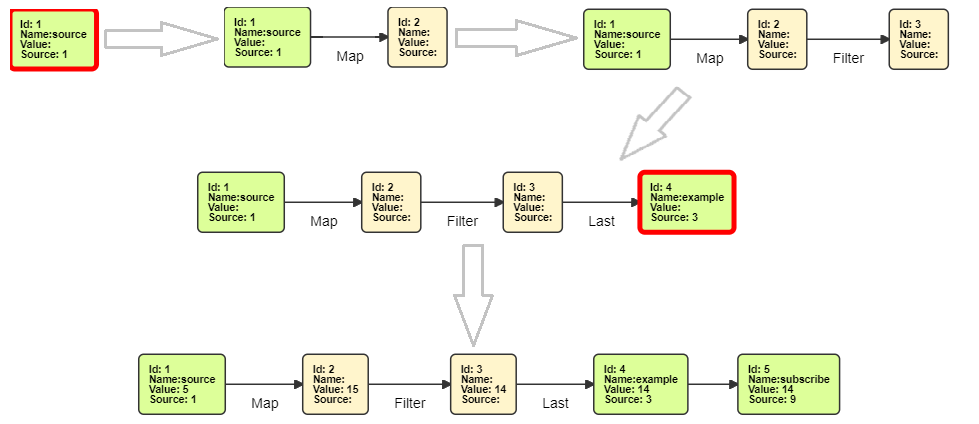
\includegraphics[scale=0.7,trim=0 0 0 0]{images/RxJS-operators/steps-all.png}
	\caption{Dependency graph evolution - RxJS Operators example}
	\label{fig:rxjs-operators-dg-evolution}
\end{figure}

\section{RxJS - Subjects}
Listing \ref{lst:rxjs-data-binding} shows relevant javascript code for this example. In current example, user enters data in two HTML input fields: firstname and lastname. Output of the application is the combination of both names. The UI of an application looks as shown in figure~\ref{fig:sd-ui} and dependency graph is shown in figure~\ref{fig:sd-dg}. 

\begin{lstlisting}[language=JavaScript, caption=RxJS - Databinding example, label={lst:rxjs-data-binding}]
// Create simple bindings for first and last name
var firstName1 = new Rx.BehaviorSubject('');
var lastName1 = new Rx.BehaviorSubject('');

// Create first and last name composite
var fullName1 = firstName1.combineLatest(lastName1, function (first, last) {
	return first + ' ' + last;
});

// Subscribe to them all
var fn1 = document.querySelector('#firstName1');
firstName1.subscribe(function (text) { fn1.value = text });

var ln1 = document.querySelector('#lastName1');
lastName1.subscribe(function (text) { ln1.value = text });

var full1 = document.querySelector('#fullName1');
fullName1.subscribe(function (text) { full1.value = text });

// Create two way bindings for both first name and last name
Rx.Observable.fromEvent(fn1, 'keyup')
.subscribe(function (e) { firstName1.next(e.target.value); })

Rx.Observable.fromEvent(ln1, 'keyup')
.subscribe(function (e) { lastName1.next(e.target.value); })
\end{lstlisting}


\begin{figure}[!h]
	\centering
	\subfloat[UI]{\includegraphics[width=0.4\textwidth]{images/simple-data-binding/simple-db-UI.png}\label{fig:sd-ui}}
	\hfill
	\subfloat[Dependency graph]{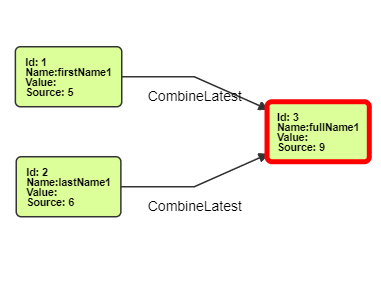
\includegraphics[width=0.4\textwidth]{images/simple-data-binding/sd-dg.png}\label{fig:sd-dg}}
	\caption{Simple Data-binding example - RxJS}
\end{figure}

\section{RxJS - Animation Test}
This is a simple animation example in which the user moves the mouse in the given area and the mouse trail with colorful boxes is animated. Relevant code for the example is listed in the listing \ref{lst:rxjs-animation-test}. This kind of example is hard to implement with vanilla javascript. Thankfully RxJS does all the work for user and emits mouse pointer values in the form of data streams. UI for the example is depicted in figure \ref{fig:rxjs-at-ui} and dependency graph generated is shown in figure \ref{fig:rxjs-at-dg}.

\begin{lstlisting}[language=JavaScript, caption=RxJS - Animation Test example, label={lst:rxjs-animation-test}]	
$(function () {
	Rx.Observable.prototype.movingWindow = function(size, selector, onShift) {
		var source1 = this;
		return Rx.Observable.create(function (o) {
			var arr = [];
			return source1.subscribe(
			function (x) {
				var item = selector(x);
				arr.push(item);
				if (arr.length > size) {
					var i = arr.shift();
					onShift(i);
				}
			},
			function (e) { o.onError(e); }
			);
		})
	}
	// Drawing area
	var canvas = $('#drawing');
	var source = Rx.Observable.fromEvent(canvas, 'mousemove')
	.movingWindow(
	25,
	function (x) {
		var b = new Box([x.clientX, x.clientY], canvas);
		b.showBox();
		return b;
	},
	function (b) {
		b.hideBox();
	}
	);	
	var sourceSubscriber = source.subscribe();	
});
\end{lstlisting}

\begin{figure}[!h]
	\centering
	\includegraphics[scale=0.4,trim=0 0 0 0]{images/animation-test/at-ui.png}
	\caption{UI - Animation Test}
	\label{fig:rxjs-at-ui}
\end{figure}
\begin{figure}[!h]
	\centering
	\includegraphics[scale=0.4,trim=0 0 0 0]{images/animation-test/at-dg.png}
	\caption{Dependency graph - Animation Test}
	\label{fig:rxjs-at-dg}
\end{figure}

\section{RxJS - Drawing example}
This is one of the advanced example from the previous examples. Figure \ref{fig:rxjs-draw-ui} shows the options available for the user. Here, the user has seven different options to draw an image. User can set outer-radius, inner-radius, different color fillings to an image. As soon as user modifies the value from the available options, the same is reflected in the image. The relevant dependency graph is shown in figure \ref{fig:rxjs-draw-dg}.

\begin{figure}[!h]
	\centering
	\includegraphics[scale=0.5,trim=0 0 0 0]{images/draw/draw-ui.png}
	\caption{UI - Drawing example}
	\label{fig:rxjs-draw-ui}
\end{figure}

\begin{lstlisting}[language=JavaScript, caption=RxJS - Drawing example, label={lst:rxjs-draw}]
var Observable = Rx.Observable;
var fromEvent = Observable.fromEvent;

var points$ = fromEvent(points, 'input', function (e) {
	return e.target.value;
}).startWith(points.value);

var outerRadius$ = fromEvent(outerRadius, 'input', function (e) {
	return e.target.value;
}).startWith(outerRadius.value).distinctUntilChanged();

var innerRadius$ = fromEvent(innerRadius, 'input', function (e) {
	return e.target.value;
}).startWith(innerRadius.value);

var angle$ = fromEvent(angle, 'input', function (e) {
	return e.target.value;
}).startWith(angle.value);

var lineWidth$ = fromEvent(lineWidth, 'input', function (e) {
	return e.target.value;
}).startWith(lineWidth.value);

var strokeColor$ = fromEvent(strokeColor, 'input', function (e) {
	return e.target.value;
}).startWith(strokeColor.value);

var fillColor$ = fromEvent(fillColor, 'input', function (e) {
	return e.target.value;
}).startWith(fillColor.value);

Rx.Observable.combineLatest(points$, outerRadius$, innerRadius$, angle$, strokeColor$, fillColor$, lineWidth$).subscribe(function (values) {
	draw.apply(null, values);
});

\end{lstlisting}

Listing \ref{lst:rxjs-draw} shows relevant RxJS code for the example. It looks complicated at the first glance. But with the help of dependency graph, user can understand which part of the code depends on other part of the code. 

\begin{figure}[!h]
	\centering
	\includegraphics[width=\textwidth,height=\textheight,keepaspectratio]{images/draw/draw-dg.png}
	\caption{Dependency graph - Drawing example}
	\label{fig:rxjs-draw-dg}
\end{figure}

We will evaluate breakpoint feature of CRI extension against this example. In large applications, it is important for the user to know at what point of the program bug exists. Breakpoint feature helps user to find out by specifying conditions. In our example, we will set up a breakpoint when node with ID 19 is created. We select \textit{nodeCreated[nodeId]} from the dropdown available, which is discussed in~\ref{section:cri-ui} and set value to \textit{nodeCreated[19]}. After setting up breakpoint, the user can see all the breakpoints as shown in figure \ref{fig:rxjs-draw-bp}. Figure \ref{fig:rxjs-draw-bp} and \ref{fig:rxjs-draw-bp2} shows that when a program hits the breakpoint, it halts the execution and goes into debugger mode. 

\begin{figure}[h]
	\centering
	\includegraphics[width=\textwidth,height=\textheight,keepaspectratio]{images/draw/breakpoint-example-1.png}
	\caption{Setup Breakpoint - Drawing example}
	\label{fig:rxjs-draw-bp}
\end{figure}

\begin{figure}[h]
	\centering
	\includegraphics[width=\textwidth,height=\textheight,keepaspectratio]{images/draw/breakpoint-example-2.png}
	\caption{After Breakpoint is hit}
	\label{fig:rxjs-draw-bp2}
\end{figure}


\section{RxJS - Stopwatch example}
Let us have a look at another typical example from RxJS applications. This application acts as a stopwatch with initial time of 90 seconds. When a user clicks on the timer, counter starts. When user clicks on running timer, it is paused. Listing \ref{lst:rxjs-stopwatch} shows relevant RxJS code for the application. And figure \ref{fig:rxjs-sw-dg} shows dependency graph generated for the application. In this example, there are 17 operators in total. Among them, 9 unique operators used. 

%\begin{sidewaysfigure}[!ht]
%	\centering
%	\includegraphics[width=\textwidth]{images/stopwatch/stopwatch-dg.png}
%	\caption{Dependency graph - Stopwatch}
%	\label{fig:rxjs-sw-dg}
%\end{sidewaysfigure}
\begin{figure}[!h]
	\centering
	\includegraphics[width=\textwidth,height=\textheight,keepaspectratio]{images/draw/draw-dg.png}
	\caption{Dependency graph - Drawing example}
	\label{fig:rxjs-sw-dg}
\end{figure}

\begin{lstlisting}[language=JavaScript, caption=RxJS - Stopwatch example, label={lst:rxjs-stopwatch}]
// DOM elements

var interval$ = Rx.Observable.interval(1000);
var click$ = Rx.Observable.fromEvent(document, 'click');
var dblclick$ = Rx.Observable.fromEvent(document, 'dblclick');
var toggleOrReset$ = Rx.Observable.merge(click$.mapTo(function (isRunning) {
	return !isRunning;
}), dblclick$.mapTo(function () {
	return false;
})).startWith(false).scan(function (isRunning, toggleOrFalse) {
	return toggleOrFalse(isRunning);
}).do(function (isRunning) {
	return console.log('Running:', isRunning);
}).share();
var start$ = toggleOrReset$.filter(function (isRunning) {
	return isRunning;
});
var stop$ = toggleOrReset$.filter(function (isRunning) {
	return !isRunning;
});
var incOrDecOrReset$ = Rx.Observable.merge(interval$.takeUntil(Rx.Observable.merge(stop$, dblclick$)).mapTo(incOrDec), dblclick$.mapTo(reset));
start$.switchMapTo(incOrDecOrReset$).startWith(initialValue).scan(function (seconds, incOrDecOrReset) {
	return incOrDecOrReset(seconds);
}).takeWhile(stillCan).map(toTime).subscribe(render);

\end{lstlisting}


We will evaluate CRI features such as search, find dependents and dependencies of a given node against this application. Similarly, user can use these features for all the RxJS applications. 
For example, we will search node named \textit{toggleOrReset\$} in the dependency graph. Figure \ref{fig:stopwatch-search} depicts the result of the search. This features makes navigation in large dependency graphs much comfortable.

\begin{figure}[!h]
	\centering
	\includegraphics[width=\textwidth,height=\textheight,keepaspectratio]{images/stopwatch/search.png}
	\caption{Search feature}
	\label{fig:stopwatch-search}
\end{figure}

Dependency highlighting feature helps the user to find all the dependents and dependencies of a given node much easier. Figure \ref{fig:dependents} shows all the dependent nodes and figure \ref{fig:dependencies} highlights all the dependency nodes of given node \textit{toggleOrReset\$}.  

\begin{figure}[!h]
	\centering
	\includegraphics[width=\textwidth,height=\textheight,keepaspectratio]{images/stopwatch/dependents.png}
	\caption{Highlighting Dependent nodes}
	\label{fig:dependents}
\end{figure}

\begin{figure}[!h]
	\centering
	\includegraphics[width=\textwidth,height=\textheight,keepaspectratio]{images/stopwatch/dependencies.png}
	\caption{Highlighting dependencies of a node}
	\label{fig:dependencies}
\end{figure}

\section{BaconJS - Drag-n-Drop}
Let us look into another interesting application called ``Drag-n-Drop''. When uploading files to server via browser, some websites provide an option to drag and drop the files. Our application imitates such feature but not with files. In this application, the user can drag contents from one box and drop in another box. For example, in the figure \ref{fig:drag-drop-ui}, last box contains both \textbf{A} and \textbf{B} values. User can drop \textbf{B} in box B but not in A. Similarly, \textbf{A} can be dropped in box A only. Listing \ref{lst:drag-drop-code}, shows relevant code for the example. Figure \ref{fig:drag-drop-dg}, depicts final view of the dependency graph.

\begin{figure}[!h]
	\centering
	\includegraphics[width=\textwidth,height=\textheight,keepaspectratio]{images/drag-drop/drag-drop-ui.png}
	\caption{BaconJS - Drag-n-Drop UI}
	\label{fig:drag-drop-ui}
\end{figure}

\begin{figure}[!h]
	\centering
	\includegraphics[width=\textwidth,height=\textheight,keepaspectratio]{images/drag-drop/drag-drop-dg.png}
	\caption{BaconJS - Drag-n-Drop Dependency graph}
	\label{fig:drag-drop-dg}
\end{figure}


\begin{lstlisting}[language=JavaScript, caption=BaconJS - Drag-n-Drop Example, label={lst:drag-drop-code}]
var homeBin, drag, drop, this$ = this;
$.event.props.push('dataTransfer');
homeBin = $('#home-bin');
drag = $(document).asEventStream('dragstart', '.item').doAction(function (e) {
	e.dataTransfer.effectAllowed = 'move';
	return e.dataTransfer.setData('tmp', '');
	}).toProperty();
drop = $('.drag-bin').asEventStream('dragover drop').doAction(function (it) {
	return it.preventDefault();
	}).filter(function (it) {
		return it.type === 'drop';
}).toProperty();
drag.combine(drop, function (a, b) {
return [a, b];
}).filter(function (arg$) {
var a, b;
a = arg$[0], b = arg$[1];
return a.timeStamp < b.timeStamp;
}).map(function (arg$) {
var a, b;
a = arg$[0], b = arg$[1];
return {
item: a.target,
dest: b.target
};
}).filter(function (arg$) {
var item, dest;
item = arg$.item, dest = arg$.dest;
return item.dataset.type === dest.dataset.type || dest.dataset.type == null;
}).assign(function (arg$) {
var item, dest;
item = arg$.item, dest = arg$.dest;
dest.appendChild(
item);
});
$('.item .remove').asEventStream('click').assign(function (e) {
homeBin.append(
$(e.target).closest('.item'));
});
\end{lstlisting}

We will now evaluate \textit{History Queries} feature against this example. Use case of History queries is described in the section \ref{section:cri-ui}.
After dragging \textbf{B} to box B, we ran the query \textit{nodeUpdated[drop]}. We found 2 stages where node \textit{drop} is updated. Changes after the query can be seen as shown in figure \ref{fig:drag-drop-hq}. Node \textit{drop} is updated at the step 14 and 81.  

\begin{figure}[!h]
	\centering
	\includegraphics[scale=0.7,trim=0 0 0 0]{images/drag-drop/drag-drop-hq.png}
	\caption{History Queries example}
	\label{fig:drag-drop-hq}
\end{figure}

\section{RxJS - Wikipedia updates}
Listing \ref{lst:rxjs-wiki-updates} shows a short example from RxJS applications that creates websocket connection to third party server. Server sends different type of notifications which are then received by websocket connection. The data received is then converted to data stream named \textit{updateStream}. The target application filters the \textit{updateStream} into three streams named \textit{newUserStream}, \textit{editStream} and \textit{updateCount}. Finally, values from each stream are used to draw a graph and updates other information to target web page. Dependency graph of target application is shown in the figure \ref{fig:rxjs-wiki-updates-dg} and UI is shown in figure \ref{fig:rxjs-wiki-updates-ui}. Splitting of one stream into three streams is easily understood with the help of dependency graph. Thus, helping user to quickly understand how the application is working. 

\begin{lstlisting}[language=JavaScript, caption=RxJS - Live updates from Wikipedia, label={lst:rxjs-wiki-updates}]
// Create our websocket to get wiki updates
var ws = new window.WebSocket("ws://wiki-update-sockets.herokuapp.com/");

var messageStream = fromEvent(ws, 'message');

var updateStream = messageStream.map(function(event) {
var dataString = event.data;
return JSON.parse(dataString);
});

// Filter the update stream for newuser events
var newUserStream = updateStream.filter(function(update) {
return update.type === "newuser";
});
newUserStream.subscribe(function() {
var format = d3.time.format("%X");
updateNewUser(["New user at: " + format(new Date())]);
});

// Filter the update stream for unspecified events, which we're taking to mean
// edits in this case
var editStream = updateStream.filter(function(update) {
return update.type === "unspecified";
});
editStream.subscribe(function(results) {
updateEditText(["Last edit: " + results.content]);
});

// Calculate the rate of updates over time
var updateCount = updateStream.scan(function(value) {
return ++value;
}, 0);

var sampledUpdates = updateCount.sample(Rx.Observable.interval(samplingTime));
var totalUpdatesBeforeLastSample = 0;
sampledUpdates.subscribe(function(value) {
updatesOverTime.push({
x: new Date(),
y:(value - totalUpdatesBeforeLastSample) /
(samplingTime / 1000)
});
if (updatesOverTime.length > maxNumberOfDataPoints)  {
updatesOverTime.shift();
}
totalUpdatesBeforeLastSample = value;
update(updatesOverTime);
});
\end{lstlisting}

\begin{figure}[!h]
	\centering
	\includegraphics[width=\textwidth,height=\textheight,keepaspectratio]{images/wiki-updates/wiki-updates-ui.png}
	\caption{UI - Wikipedia updates}
	\label{fig:rxjs-wiki-updates-ui}
\end{figure}
\begin{figure}[!h]
	\centering
	\includegraphics[width=\textwidth,height=\textheight,keepaspectratio]{images/wiki-updates/wiki-updates-dg.png}
	\caption{Dependency graph - Wikipedia updates}
	\label{fig:rxjs-wiki-updates-dg}
\end{figure}

\section{Existing design vs Current design}
In this section we will discuss the improvisations made in this thesis from previous version of CRI. Listing \ref{lst:rxjs-count}, shows an example which counts the length of text input from the UI~\ref{fig:rxjs-count-ui}. In line 10, we are subscribing to \textit{source} observable. Thus, every values emitted by \textit{source} is received by the subscriber and set using function \textit{setHtml} at line 5. 


\begin{lstlisting}[language=JavaScript, caption=RxJS - Letter Count, label={lst:rxjs-count}]
var source = Rx.Observable.fromEvent($toCount, 'keyup')
.map(function (e) { return 'length: ' + e.target.value.length; })
.distinctUntilChanged();

function setHtml(text) {
	console.log(text);
	this.innerHTML = text;
}

source.subscribe(setHtml.bind($result));
\end{lstlisting}

\begin{figure}[!h]
	\centering
	\includegraphics[scale=0.7,trim=0 0 0 0]{images/improvisations/initial-ui.png}
	\caption{RxJS - Letter Count example}
	\label{fig:rxjs-count-ui}
\end{figure}


In previous version of CRI developed, the author is subscribing to each observable again to catch all the events using the code listed in listing \ref{lst:prev-cri-code}. Here, \textit{obs} represents an observable from the target application. Each value emitted is then logged to dependency graph using the method \textit{sendToDevTools} at line 2. In current version, we have improved it and overridden RxJS library functions to catch all the events. Listing \ref{lst:curr-cri-code}, shows relevant code. \textit{Rx.Subscriber.prototype.next} method catches all the values emitted by all the observables from the target application. Thus, providing more control over all the emitted values and make necessary modifications. 

\begin{lstlisting}[language=JavaScript, caption=Previous implementation, label={lst:prev-cri-code}]
obs.subscribe(function (x) {
	sendObjectToDevTools({
		content: {
			'nodeId': obs.id,
			'nodeType': obsType,
			'nodeMethod': '',
			'nodeRef': '',
			'nodeValue': x,
			'sourceCodeLine': ''
		}, action: "saveNode", destination: "panel"
	});
}
\end{lstlisting}
\begin{lstlisting}[language=JavaScript, caption=Current implementation, label={lst:curr-cri-code}]
 Rx.Subscriber.prototype.next = function (value) {
 	var self = this;
 	sendObjectToDevTools({
	 	content: {
	 	'nodeId': self._id,
	 	'nodeType': self.obsType,
	 	'nodeMethod': '',
	 	'nodeRef': '',
	 	'nodeValue': value,
	 	'sourceCodeLine': ''
	 	}, action: "saveNode", destination: "panel"
 	});
 }
\end{lstlisting}

The disadvantage of previous implementation is, it logs the same values repeatedly because each observable is subscribed twice: once in target application and once in the CRI extension. This works fine for smaller application but there is huge communication overhead and excessive resource consumption. After typing the letters \textit{TU} in the text-box from figure \ref{fig:rxjs-count-ui}, total number of message communication in previous version of CRI is 36 and current version is 16. Resultant dependency graph for each version of CRI is shown in figures \ref{fig:prev-cri} and \ref{fig:curr-cri}.
There are 20 extra message communications, which consumes resources to communicate. The numbers vary to large extent in bigger applications. And current version of CRI provide more detailed information regarding what is going on in the target application. For example, look at the node with id 1, in both the figures \ref{fig:prev-cri} and \ref{fig:curr-cri}. As the user types, CRI catches the events and maps them to display meaningful data to help the developers. 

\begin{figure}[!h]
	\centering
	\includegraphics[width=\textwidth,height=\textheight,keepaspectratio]{images/improvisations/previous.png}
	\caption{CRI - Previous version}
	\label{fig:prev-cri}
\end{figure}
\begin{figure}[!h]
	\centering
	\includegraphics[width=\textwidth,height=\textheight,keepaspectratio]{images/improvisations/new.png}
	\caption{CRI - Current version}
	\label{fig:curr-cri}
\end{figure}

\section{Profiling Time - Library calls from the User space}
In this section we evaluate time taken by overridden RxJS library function calls for the applications discussed in this chapter earlier. Google Chrome provides developers the performance API - Google Chrome DevTools \textbf{Javascript Profiler}\cite{jsprofiler}. We used this profiling feature to evaluate performance of CRI extension. Javascript profiler provides more detailed information on which javascript functions were called and how long each took. This feature from Chrome can be accessed by navigating to DevTools and select the panel ``Javascript Profiler''. Then, user can click on start button to start the recording and upon stopping, the user can see the snapshot of the functions that were called and the time each function took. The figures \ref{fig:prof-without-cri} and \ref{fig:prof-with-cri} shows the time taken by functions without CRI and with CRI used respectively. Our primary focus is on \textbf{Self-time} view. Self-time is the time on specific function and the \textbf{Total-time} is the time executing sub function calls. In CRI, we are calling original library calls in our overridden functions, \textbf{Total-time} would include the time spent in the library activities. We can see that, time spent in the functions that we have overridden is minimal in comparison.

\begin{figure}[!h]
	\centering
	\includegraphics[width=\textwidth,height=\textheight,keepaspectratio]{images/profiling/without-cri.png}
	\caption{Javascript profiling - without CRI}
	\label{fig:prof-without-cri}
\end{figure}
\begin{figure}[!h]
	\centering
	\includegraphics[width=\textwidth,height=\textheight,keepaspectratio]{images/profiling/with-cri.png}
	\caption{Javascript profiling - with CRI}
	\label{fig:prof-with-cri}
\end{figure}

\section{Summary of Evaluation}
The preceding evaluation illustrated with the help of various examples what the contributions of this thesis are. We have evaluated few other RxJS and BaconJS applications from the web and found that our extension works fine and support most of the operators from RxJS library. Additionally, we showed how visualization can help in getting good overview of reactive system and understand its internals at a glance. One main drawback of our extension is that it supports applications with javascript version upto ECMAScript 5.1\cite{es5} due to limitations of Jalangi framework\cite{jalangiissue}. Sometimes target applications have event streams which are continuously emitting values after every short interval of time, can cause heavy message passing and memory consuming. We are confident that the approach used in CRI extension works properly and helps developers to understand and debug reactive applications. 

%	\cleardoublepage
	\chapter{Conclusion and Future work} \label{chap:Summary}
In this chapter, we conclude the thesis by shortly summarising the main contributions. Additionally, various ideas for future work are introduced, so that development can proceed without any break. 

\section{Final Remarks}
The developed system is based on an already existing Chrome plugin developed at Technical University Darmstadt, which already provides the functionality to visualize dependency graph, navigating through history. The contribution of this thesis is to extend these functionalities to develop an advanced debugger and to support various RxJS operators.

The system developed in this thesis allows user to search for a particular node, to gain an understanding of its dependents and dependencies. Additionally, advanced methods to navigate the history has been developed. As shown in the evaluation, advanced debugging mechanisms for reactive programming have the potential to ease the development of reactive systems. Many ideas for further improvements are introduced in the last section.

\section{Future Work}
We believe that the CRI extension can very well be improved in the future. One aspect would be to try to instrument the javascript code using other methods such as ESPRIMA\cite{esprima} due to limitations of Jalangi framework to support latest version of javascript. A survey on, how CRI helps the developers in real time to understand the reactive applications and find bugs in them, would provide further scope for development. 

Another aspect would be to support other browsers such as Firefox and Safari. Also it would be a nice idea to integrate with NodeJS\cite{nodejs} ecosystem to debug the applications. A great help would be to improve the debugger in order to make it a so-called ``edit-and-debug''. This would give the developer the possibility to change values in dependency graph and see the output on the fly. The plugin could also provide great assistance with performance analysis. It would be a very helpful to visualize the number of times a node is evaluated. This would help developers to find the bottleneck in their code. 
%	\cleardoublepage
	
	\listoffigures
	\lstlistoflistings
%	\listoftables
	
	\printbibliography

%	\begin{appendices}
%		\chapter{APPENDIX}
\label{ch:Appendix}
\section{Ad-hoc code metrics for CRI2 and CRI3}
The lines of code include comments, lines containing only brackets and empty lines.
CRI2 has 8 own JS files with 2353 total and 294 average lines of code per file. The scripts \emph{background}, \emph{devtools} and \emph{content-script-end} are empty and were ignored for these measurements.
CRI3 has 19 own JS files with 3580 total and 188 average lines of code per file.
%%	\end{appendices}


	
\end{document}